\documentclass[tikz]{standalone}
\usepackage{tikz}

\begin{document}
\sffamily
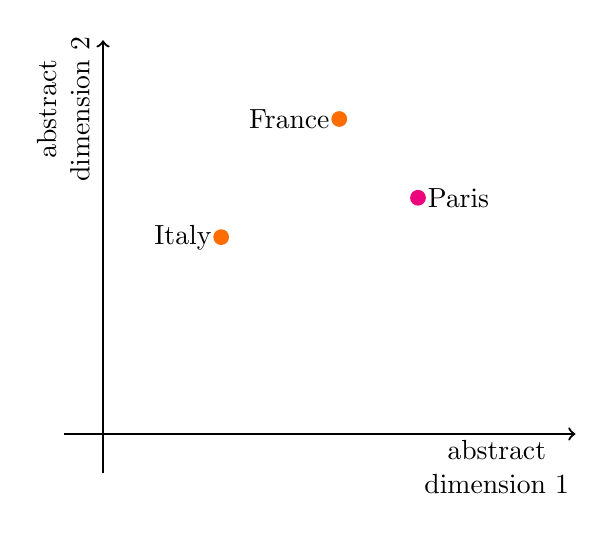
\begin{tikzpicture}
    % Draw axes
    \draw[thick, ->] (-0.5, 0) -- (6, 0) ;
    \node at (5.0, -1.0)  [label={[align=center]abstract\\dimension 1}] {};
    
    \draw[thick, ->] (0, -0.5) -- (0, 5);
    \node at (-0.05, 4) [label={[rotate=90,align=center]abstract\\dimension 2}] {};

    \coordinate (france) at (3,4);
    \coordinate (italy) at (1.5,2.5);
    \coordinate (paris) at (4,3);
    \coordinate (rome) at (2.5,1.5);
    
    \fill[orange!85!red] (france) circle (0.1);
    \node[left] at (france) {France};
    \fill[orange!85!red] (italy) circle (0.1);
    \node[left] at (italy) {Italy};
    \fill[magenta!85!red] (paris) circle (0.1);
    \node[right] at (paris) {Paris};
    %\fill[magenta!85!red] (rome) circle (0.1);
    %\node[right] at (rome) {Rome};

    %\draw[very thick, black, -latex] (france) -- (paris);
    %\draw[very thick, black, -latex] (italy) -- (rome);
    
\end{tikzpicture}

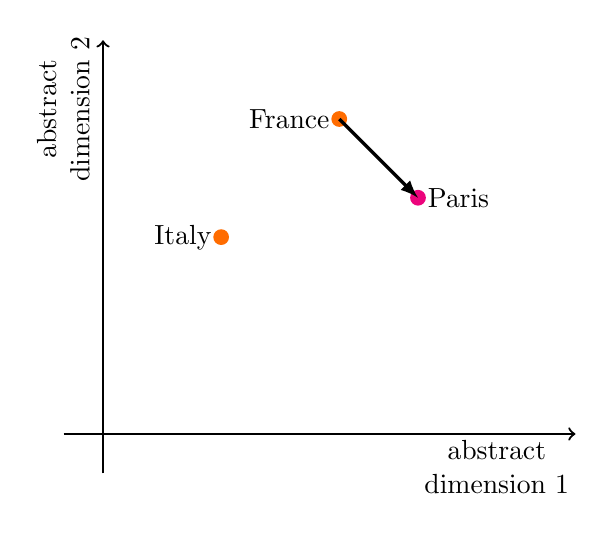
\begin{tikzpicture}
    % Draw axes
    \draw[thick, ->] (-0.5, 0) -- (6, 0) ;
    \node at (5.0, -1.0)  [label={[align=center]abstract\\dimension 1}] {};
    
    \draw[thick, ->] (0, -0.5) -- (0, 5);
    \node at (-0.05, 4) [label={[rotate=90,align=center]abstract\\dimension 2}] {};

    \coordinate (france) at (3,4);
    \coordinate (italy) at (1.5,2.5);
    \coordinate (paris) at (4,3);
    \coordinate (rome) at (2.5,1.5);
    
    \fill[orange!85!red] (france) circle (0.1);
    \node[left] at (france) {France};
    \fill[orange!85!red] (italy) circle (0.1);
    \node[left] at (italy) {Italy};
    \fill[magenta!85!red] (paris) circle (0.1);
    \node[right] at (paris) {Paris};
    %\fill[magenta!85!red] (rome) circle (0.1);
    %\node[right] at (rome) {Rome};

    \draw[very thick, black, -latex] (france) -- (paris);
    %\draw[very thick, black, -latex] (italy) -- (rome);
    
\end{tikzpicture}

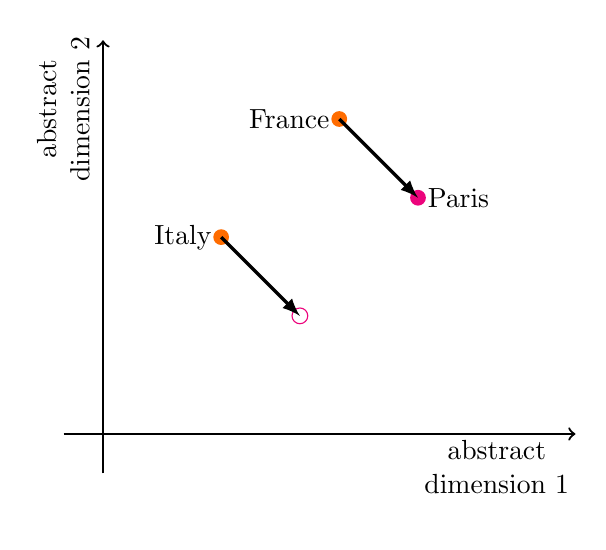
\begin{tikzpicture}
    % Draw axes
    \draw[thick, ->] (-0.5, 0) -- (6, 0) ;
    \node at (5.0, -1.0)  [label={[align=center]abstract\\dimension 1}] {};
    
    \draw[thick, ->] (0, -0.5) -- (0, 5);
    \node at (-0.05, 4) [label={[rotate=90,align=center]abstract\\dimension 2}] {};

    \coordinate (france) at (3,4);
    \coordinate (italy) at (1.5,2.5);
    \coordinate (paris) at (4,3);
    \coordinate (rome) at (2.5,1.5);
    
    \fill[orange!85!red] (france) circle (0.1);
    \node[left] at (france) {France};
    \fill[orange!85!red] (italy) circle (0.1);
    \node[left] at (italy) {Italy};
    \fill[magenta!85!red] (paris) circle (0.1);
    \node[right] at (paris) {Paris};
    \draw[magenta!85!red] (rome) circle (0.1);
    %\node[right] at (rome) {Rome};

    \draw[very thick, black, -latex] (france) -- (paris);
    \draw[very thick, black, -latex] (italy) -- (rome);
\end{tikzpicture}

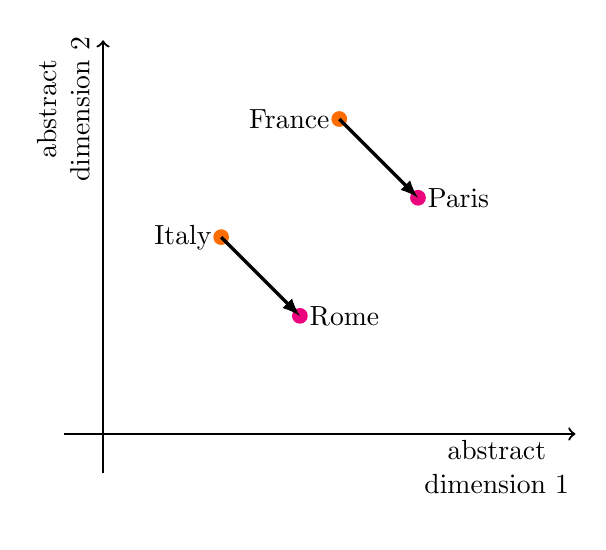
\begin{tikzpicture}
    % Draw axes
    \draw[thick, ->] (-0.5, 0) -- (6, 0) ;
    \node at (5.0, -1.0)  [label={[align=center]abstract\\dimension 1}] {};
    
    \draw[thick, ->] (0, -0.5) -- (0, 5);
    \node at (-0.05, 4) [label={[rotate=90,align=center]abstract\\dimension 2}] {};

    \coordinate (france) at (3,4);
    \coordinate (italy) at (1.5,2.5);
    \coordinate (paris) at (4,3);
    \coordinate (rome) at (2.5,1.5);
    
    \fill[orange!85!red] (france) circle (0.1);
    \node[left] at (france) {France};
    \fill[orange!85!red] (italy) circle (0.1);
    \node[left] at (italy) {Italy};
    \fill[magenta!85!red] (paris) circle (0.1);
    \node[right] at (paris) {Paris};
    \fill[magenta!85!red] (rome) circle (0.1);
    \node[right] at (rome) {Rome};

    \draw[very thick, black, -latex] (france) -- (paris);
    \draw[very thick, black, -latex] (italy) -- (rome);
    
\end{tikzpicture}
\end{document}

